\documentclass[a4paper]{article}

% Increase text width
\usepackage[left=48pt,right=46pt]{geometry}

% Images Stuff
\usepackage{graphicx} % Required to insert images
\usepackage{float} % Used to position images
\graphicspath{ {images/} }

% Uncomment for no indent at start of paragraphs
%\setlength\parindent{0pt} % no indent for new paragraphs


\usepackage{hyperref} % Makes toc, urls, figure links

% format hyperlinks nicer than default way
\usepackage{xcolor}
\hypersetup{colorlinks,linkcolor={blue!80!black},citecolor={blue!80!black},urlcolor={blue!80!black}}

% Use to embed code
\usepackage{listings}
\lstset{
  basicstyle=\ttfamily,
  columns=fullflexible,
  frame=single,
  breaklines=true,
  postbreak=\mbox{\space},
  aboveskip=20pt,
  belowskip=20pt,
  showstringspaces=false
}

% Change caption title for lslistings
\renewcommand{\lstlistingname}{Code Sample}

\usepackage[title]{appendix}

% Title Page
\title{Ansible Assignment \\ \small{Cloud Infrastructure}} 

\author{Rob Shelly \\ \small{20068406}}
%\date{October 7th 2017}


\begin{document}
	
	% Title page
	\maketitle
	
	% Table of Contents
	\newpage
	\tableofcontents
	
	% Body
	\newpage
	\section{Introduction}
    The document will outline the concepts behind and the tasks required to configure and web server on AWS using Ansible. The web server will consist of two Nginx servers running in a private subnet, with a HAProxy load balancer running in a public subnet balancing traffic to the web servers. Also running in the public subnet is the Ansible server which will provision the Nginx and Haproxy servers. This is illustrated in \autoref{fig:diagram}. For the purposes of this exercise, the NGinx server have been configured to redirect to \textit{serversforhackers.com}.
    
    \begin{figure}[H]
      \caption{System Architecture}
      \centering
      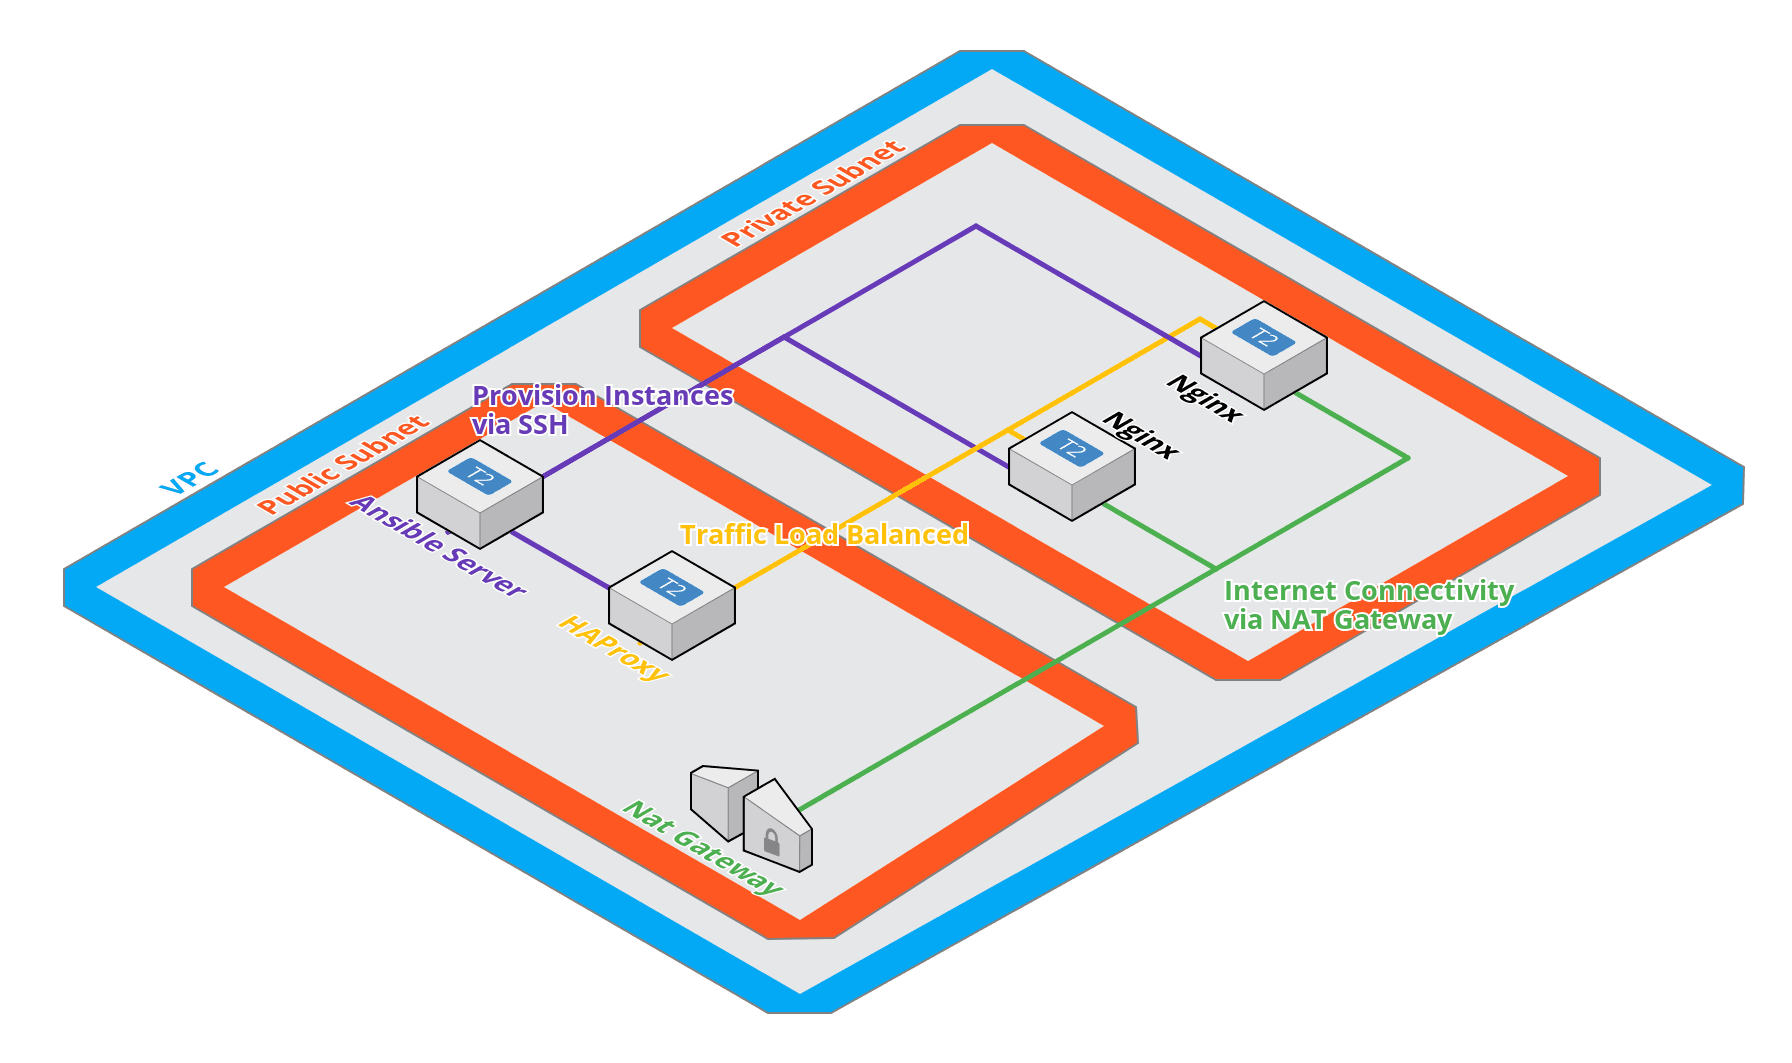
\includegraphics[width=\textwidth,height=\textheight,keepaspectratio]{diagram1}
      \label{fig:diagram}
    \end{figure}
    
  \section{Ansible}
    Ansible configures servers though the use of a number of key concepts, the first of which is \textit{Playbooks}. Playbooks define the configuration to be deployed to a server. When executed against a server they run a number of tasks which will make the necessary installations, create the necessary file etc. to configure the server. The are also idempotent, meaning that can be run multiple times without changing or breaking the initial result.
    
    Playbooks use \textit{tasks} and \textit{handlers} to configure servers. Tasks are the individual steps required for configuration, such as adding a package repository or installing a package. When a playbook is run, all of it's tasks are executed in order. Handlers, however are only executed when called. For example a handler to start a service might be called after installing the service.
  
    Writing the entire configuration for a server in one playbook could be quite complex and would not be very reusable. This is where \textit{roles} are used. Roles group task, handlers and other files such as variable files and templates together in a standard directory structure. A role can then be called by a playbook. A role can even be called but instructed to use a different variable file. This allows for greater reuse in Ansible. 
  
  \section{Roles}
  In order to deploy the system described above, Ansible must create EC2 instances within the VPC, then provision the necessary servers with Nginx or HAProxy. Therefore, three roles will be used to create this system:
  
  \begin{itemize}
    \item Provision EC2 Instance
    \item Nginx
    \item HAProxy
  \end{itemize}
  
    \subsection{Provision EC2 Instance}
    This roles is used to provision an instances within EC2. The roles defines three main tasks:
    \begin{itemize}
      \item Provision the instance(s)
      \item Add the instances to the dynamic list of hosts held by ansible
      \item Wait for the instance(s) to be reachable via SSH
    \end{itemize}
    These tasks are shown below \autoref{provision-tasks}. There are a number of aspect to note in these tasks.
    \begin{itemize}
      \item There are a large number of variables included in the tasks. This will allow the role to be reused. For example, the \textit{instance\_count} will allow the role to be used to create two Nginx servers initially but only one HAProxy server later.
      \item The task adds the instance(s) it created to a group in the hosts files, defined by the \textit{host\_group} variable. The means that instances create by the role can then be provisions with the correct configuration by running playbooks against the hosts in the \textit{host\_group}
      \item The task add the private IP addresses of the instance to the hosts file. This is necessary because some of the server are created in a private subnet and therefore have no public IP address. However, as the Ansible server is running in the public subnet, it can connect to any server in either the private or public subnets using their private IP addresses.
    \end{itemize}
    
    \noindent In order to use the role ro provision server differently, (i.e. for Nginx server or a HAProxy server) two different variable files are defined; \textit{webserver.yml} and \textit{loadbalancer.yml}. This are shown in appendix \ref{provision-vars}.
    
		\begin{minipage}{\textwidth}
      \begin{lstlisting}[caption={provision-ec2-instance/tasks/main.yml},label=provision-tasks,language=bash]
      ---
      - name: Provision EC2 Box
      local_action:
      module: ec2
      profile: "{{ aws_profile }}"
      key_name: "{{ ec2_keypair }}"
      group_id: "{{ ec2_security_group }}"
      instance_type: "{{ ec2_instance_type }}"
      image: "{{ ec2_image }}"
      vpc_subnet_id: "{{ ec2_subnet_ids|random }}"
      region: "{{ ec2_region }}"
      instance_tags: '{"Name":"{{ec2_tag_Name}}","Type":"{{ec2_tag_Type}}","Environment":"{{ec2_tag_Environment}}"}'
      assign_public_ip: "{{ assign_public_ip }}"
      wait: true
      count: "{{ instance_count }}"
      volumes:
      - device_name: /dev/sda1
      device_type: gp2
      volume_size: "{{ ec2_volume_size }}"
      delete_on_termination: true
      register: ec2
      
      - debug: var=item
      with_items: ec2.instances
      
      - name: Add instances to host group
      add_host:
      hostname: "{{ item.private_ip }}"
      ansible_user: "{{ ssh_user }}"
      ansible_ssh_private_key_file: "{{ ssh_key_path }}"
      ansible_python_interpreter: /usr/bin/python3
      ansible_ssh_extra_args: '-o StrictHostKeyChecking=no'
      groups: "{{ host_group }}"
      with_items: "{{ ec2.instances }}"
      
      - name: Wait for the instances to boot by checking the ssh port
      wait_for: host={{item.private_ip}} port=22 delay=60 timeout=320 state=started
      with_items: "{{ ec2.instances }}"
      \end{lstlisting}
    \end{minipage}
    
    \subsection{Nginx}
    The Nginx role consists of the following main elements:
    \begin{itemize}
      \item \textbf{Tasks:} These are the main tasks required to configure Nginx. They include adding the package repository and installing Nginx, and moving the necessary configuration files into place.
      \item \textbf{Handlers:} The Nginx role defines two handlers: \textit{Start Nginx} and \textit{Reload Nginx}. The are called as required by the main tasks. For example, after creating the Nginx configuration, the \textit{Reload Nginx} handler is called.
      \item \textbf{Templates:} Templates can be used to defined files that must be copied to the server. However they also allow for variable through the use of Jinja. The Nginx roles use a template to create the Nginx configuration file. This can be seen in  \autoref{nginx-conf-template}.
      \item \textbf{Variables:} The Nginx role also defines a variables files. In this case the web server domain is defined as a variable.
    \end{itemize}

 		\begin{minipage}{\textwidth}
      \begin{lstlisting}[caption={nginx/templates/serverforhacker.com.conf.j2},label=nginx-conf-template,language=bash]
      server {
        # Enforce the use of HTTPS
        listen 80 default_server;
        server_name {{ domain }};
        return 301 https://$server_name$request_uri;
      }
      server {
        listen 443 ssl default_server;
        root /var/www/{{ domain }}/public/;
        index index.html index.htm index.php;
        access_log /var/log/nginx/{{ domain }}.log;
        error_log /var/log/nginx/{{ domain }}-error.log error;
        server_name {{ domain }};
        charset utf-8;
        include h5bp/basic.conf;
        include h5bp/directive-only/ssl.conf;
        
        location / {
          try_files $uri $uri/ /index.php$is_args$args;
      }
        location = /favicon.ico { log_not_found off; access_log off; }
        location = /robots.txt { log_not_found off; access_log off; }
      }
      \end{lstlisting}
    \end{minipage}
    
    \subsection{HAProxy}
    The HAProxy roles is similar to the Nginx role. It defines two main tasks: \textit{Install HAProxy} and \textit{Update HAProxy Config}. Like, Nginx it also defines handlers to start and reload HAProxy. The HAProxy 
    configuration is provided by a template file. This is shown below in \autoref{haproxy-cfg}.
    
    Of particular is the \textit{server} block. This is adding the hosts in the \textit{webservers} group and their IP addresses to the HAProxy server configuration. As stated above, when the Provision EC2 Instance role runs, it adds the instance to the Ansible hosts. When run with the \textit{webservers} variables file, (which is used to provision the Nginx servers), the instances are added under the \textit{webservers} group. Therefore, this section of the template is configuring any provisioned NGinx instances as the server for HAProxy.
    
 		\begin{minipage}{\textwidth}
      \begin{lstlisting}[caption={haproxy/templates/haproxy.cfg},label=haproxy-cfg,language=bash]
        global
          log 127.0.0.1 local0 notice
          maxconn 2000
          user haproxy
          group haproxy
        
        defaults
          log     global
          mode    http
          option  httplog
          option  dontlognull
          retries 3
          option redispatch
          timeout connect  5000
          timeout client  10000
          timeout server  10000
        
        listen {{haproxy_app_name}} 
          bind 0.0.0.0:80
          mode {{haproxy_mode}}
          stats {{haproxy_enable_stats}}
          
          stats uri /haproxy_stats
          stats realm Strictly\ Private
          
          stats auth {{user.username}}:{{user.password}}
          
          
          balance {{haproxy_algorithm}}
          option httpclose
          option forwardfor 
          
          
          server {{hostvars[host]['ansible_hostname']}} {{ hostvars[host]['ansible_eth0']['ipv4']['address'] }}:80 check
          
      \end{lstlisting}
    \end{minipage}
    
  \section{Playbooks}
    With all the roles defined, playbooks can be created to run these roles against the necessary servers. Although one playbook could be created to run each of the roles, it is preferable to create multiple playbooks for each of the server to be configured and include these in one \textit{master} playbook. These playbooks are included in appendix \ref{playbooks}.
    The playbooks are then called from one master playbook, shown below in \autoref{playbook}
    
    \noindent
    \begin{minipage}{\textwidth}
      \begin{lstlisting}[caption={main-playbook.yml},label=playbook,language=bash]
        ---
        - import_playbook: provision-ec2.yml type='webservers'
        - import_playbook: nginx.yml hosts='webservers'
        - import_playbook: provision-ec2.yml type='loadbalancer'
        - import_playbook: haproxy.yml hosts='loadbalancer'
      \end{lstlisting}
    \end{minipage}
    
    \noindent Here, the Provision EC2 playbook is called twice. However, in order to deploy the different instances (i.e. two in the private subnet for Nginx, one in the public subnet for HAProxyy), the \textit{type} variable is used to specify which variables files should be used. Also, the \textit{hosts} variables are used to instruct the Nginx and HAProxy playbooks which server they should run against.
    
  \section{Ansible Vault}
  Each of the roles have specified variable files. These have been used to allow for greater reuse of the roles. However, they can also contain sensitive information. Ansible Vault provides a method of encrypting these files while still allowing them to be used by playbooks, by providing a password. All of the variable files were encrypted using the following command:
  
  \noindent
  \begin{minipage}{\textwidth}
    \begin{lstlisting}[caption={vault.yml},label=vault,language=bash]
      ansible-vault encrypt roles/<rolename>/vars/<filename>
    \end{lstlisting}
  \end{minipage}
  
  \noindent They can also be edited or decrypted using the \textit{edit} and \textit{decrypt} flags.
  
  \section{Running the Playbook}
  The \textit{main-playbook} can now be run. However, Ansible must have SSH access to the server it created in the private subnet in order to install Nginx on them. Therefore, the playbook was run on the Ansible server within the VPC, specifically within the public subnet. The following command runs the playbook, asking the user to enter their password to use the variable files encrypted by Ansible vault.
  
  \noindent
  \begin{minipage}{\textwidth}
    \begin{lstlisting}[caption={run.yml},label=run,language=bash]
      ansible-playbook --ask-vault-pass -i localhost, main-playbook.yml
    \end{lstlisting}
  \end{minipage}
  
  Once the playbook visiting the AWS console verified that the correct instances have been created, shown in \autoref{aws}. Note that the Nginx server have no public IP addresses as they are within the private subnet.
  
  \begin{figure}[H]
    \caption{EC2 Instance}
    \centering
    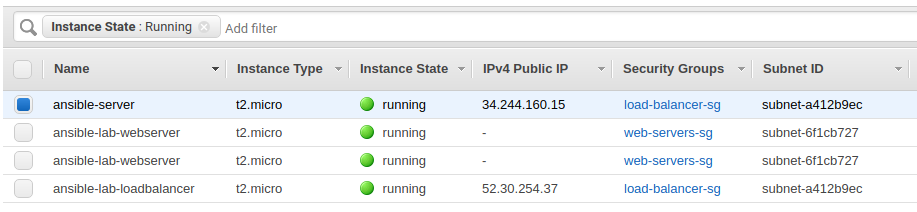
\includegraphics[width=\textwidth,height=\textheight,keepaspectratio]{aws}
    \label{fig:aws}
  \end{figure}
  
  By visiting the \textit{stats} page of the HAProxy server the status of the two web servers can be verified.
  
  \begin{figure}[H]
    \caption{HAProxy}
    \centering
    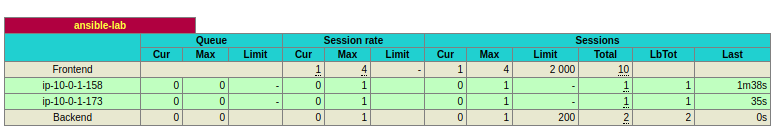
\includegraphics[width=\textwidth,height=\textheight,keepaspectratio]{haproxy}
    \label{fig:haproxy}
  \end{figure}
  
  \begin{appendices}
    \section{Project Repository} \label{code}
Relevant code samples have been provided in this document. However the project in it's entirety can be found at the following link:

\noindent \href{https://github.com/robshelly/ansible-lab}{https://github.com/robshelly/ansible-lab}
    \section{Provision EC2 Instance Variable files} \label{provision-vars}

\begin{minipage}{\textwidth}
  \begin{lstlisting}[caption={provision-ec2-instance/vars/webserver.yml},label=webserver-vars,language=bash]
  ---
  ec2_keypair: "ansible"
  ec2_security_group: "sg-73dbc209"
  ec2_instance_type: "t2.micro"
  ec2_image: "ami-f90a4880"
  ec2_subnet_ids: ['subnet-6f1cb727']
  ec2_region: "eu-west-1"
  ec2_tag_Name: "ansible-lab-webserver"
  ec2_tag_Type: "ansible-lab-webserver"
  ec2_tag_Environment: "production"
  ec2_volume_size: 8
  assign_public_ip: no
  host_group: webservers
  instance_count: 2
  ssh_user: ubuntu
  ssh_key_path: ~/keypairs/ansible.pem
  aws_profile: ansible
\end{lstlisting}
\end{minipage}


\noindent
\begin{minipage}{\textwidth}
  \begin{lstlisting}[caption={provision-ec2-instance/vars/loadbalance.yml},label=loadbalancer-vars,language=bash]
  ---
  ec2_keypair: "ansible"
  ec2_security_group: "sg-6cdcc516"
  ec2_instance_type: "t2.micro"
  ec2_image: "ami-f90a4880"
  ec2_subnet_ids: ['subnet-a412b9ec']
  ec2_region: "eu-west-1"
  ec2_tag_Name: "ansible-lab-loadbalancer"
  ec2_tag_Type: "ansible-lab-loadbalancer"
  ec2_tag_Environment: "production"
  ec2_volume_size: 8
  assign_public_ip: yes
  host_group: loadbalancer
  instance_count: 1
  ssh_user: ubuntu
  ssh_key_path: ~/keypairs/ansible.pem
  aws_profile: ansible
  \end{lstlisting}
\end{minipage}
    \section{Provision EC2 Instance Variable files} \label{playbooks}

\begin{minipage}{\textwidth}
  \begin{lstlisting}[caption={provision-ec2.yml},label=ec2-playbook,language=bash]
    ---
    - hosts: localhost
    connection: local
    gather_facts: false
    user: root
    pre_tasks:
    - include_vars: ~/ansible-lab/roles/provision-ec2-instance/vars/{{type}}.yml
    roles:
    - provision-ec2-instance
  \end{lstlisting}
\end{minipage}

\noindent
\begin{minipage}{\textwidth}
  \begin{lstlisting}[caption={nginx.yml},label=nginx-playbook,language=bash]
    ---
    - hosts: "{{hosts}}"
    become: yes
    become_user: root
    roles:
    - nginx
  \end{lstlisting}
\end{minipage}

\noindent
\begin{minipage}{\textwidth}
  \begin{lstlisting}[caption={haproxy.yml},label=haproxy-playbook,language=bash]
    ---
    - hosts: "{{hosts}}"
    become: yes
    become_user: root
    roles:
    - haproxy
  \end{lstlisting}
\end{minipage}
  \end{appendices}
    
	
\end{document}
        
